\documentclass{standalone}
\usepackage{graphicx, standalone}
\usepackage[compat=1.1.0]{tikz-feynman}
\usepackage{tikz}
\usepackage{amsmath, amssymb}
\usepackage{euler}
\usepackage{fontspec}
\setmainfont{MinionPro}
\usepackage{comment}

\renewcommand{\k}{\ensuremath\text{k}}
\newcommand{\kp}{\ensuremath\text{k}'}
\newcommand{\q}{\ensuremath\text{q}}

\begin{document}
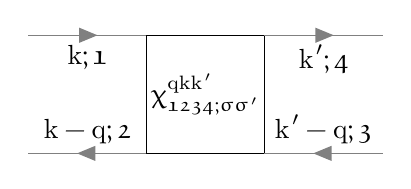
\begin{tikzpicture}[baseline=(current bounding box.center)]
\begin{feynman}
	\vertex (a1);
	\vertex[below=of a1] (a2);
	\vertex[right=of a1] (b1);
	\vertex[below=of b1] (b2);
	\vertex[right=of b1] (c1);
	\vertex[below=of c1] (c2);
	\vertex[right=of c1] (d1);
	\vertex[below=of d1] (d2);

	\node (content) at ($(b1)!0.5!(c2)$) {$\chi^{\q\k\kp}_{\mathfrak{1234};\sigma\sigma'}$};	
	
	\diagram* {
		(b1) -- (c1) -- (c2) -- (b2) -- (b1),
		(a1) -- [fermion, gray, edge label'=$\k;\mathfrak{1}$, text=black] (b1),
		(b2) -- [fermion, gray, edge label'=$\k-\q;\mathfrak{2}$, text=black] (a2),
		(d2) -- [fermion, gray, edge label'=$\k'-\q;\mathfrak{3}$, text=black] (c2),
		(c1) -- [fermion, gray, edge label'=$\k';\mathfrak{4}$, text=black] (d1),
	};
\end{feynman}
\end{tikzpicture}
\begin{tikzpicture}[baseline=(current bounding box.center)]
	\node {$=$};
\end{tikzpicture}
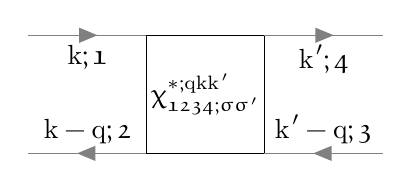
\begin{tikzpicture}[baseline=(current bounding box.center)]
\begin{feynman}
	\vertex (a1);
	\vertex[below=of a1] (a2);
	\vertex[right=of a1] (b1);
	\vertex[below=of b1] (b2);
	\vertex[right=of b1] (c1);
	\vertex[below=of c1] (c2);
	\vertex[right=of c1] (d1);
	\vertex[below=of d1] (d2);

	\node (content) at ($(b1)!0.5!(c2)$) {$\chi^{*;\q\k\kp}_{\mathfrak{1234};\sigma\sigma'}$};	
	
	\diagram* {
		(b1) -- (c1) -- (c2) -- (b2) -- (b1),
		(a1) -- [fermion, gray, edge label'=$\k;\mathfrak{1}$, text=black] (b1),
		(b2) -- [fermion, gray, edge label'=$\k-\q;\mathfrak{2}$, text=black] (a2),
		(d2) -- [fermion, gray, edge label'=$\k'-\q;\mathfrak{3}$, text=black] (c2),
		(c1) -- [fermion, gray, edge label'=$\k';\mathfrak{4}$, text=black] (d1),
	};
\end{feynman}
\end{tikzpicture}
\begin{tikzpicture}[baseline=(current bounding box.center)]
	\node {$-$};
\end{tikzpicture}
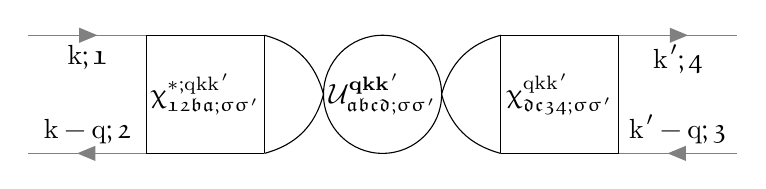
\begin{tikzpicture}[baseline=(current bounding box.center)]
\begin{feynman}
	\vertex (a1);
	\vertex[below=of a1] (a2);
	\vertex[right=of a1] (b1);
	\vertex[below=of b1] (b2);
	\vertex[right=of b1] (c1);
	\vertex[below=of c1] (c2);
	\vertex[right=of c1] (d1);
	\vertex[below=of d1] (d2);
	\vertex[right=of d1] (e1);
	\vertex[below=of e1] (e2);
	\vertex[right=of e1] (f1);
	\vertex[below=of f1] (f2);
	\vertex[right=of f1] (g1);
	\vertex[below=of g1] (g2);

	\node (content1) at ($(b1)!0.5!(c2)$) {$\chi^{*;\q\k\kp}_{\mathfrak{12ba};\sigma\sigma'}$};	
	\node (content2) at ($(e1)!0.5!(f2)$) {$\chi^{\q\k\kp}_{\mathfrak{dc34};\sigma\sigma'}$};
	
	\vertex (u1) at ($(c1)+(0.75,-0.75)$);
	\vertex (u2) at ($(u1)+(1.5,0)$);
	\vertex (u) at ($(u1)!0.5!(u2)$) {$\mathcal{U}^{\textbf{qkk}'}_{\mathfrak{abcd};\sigma\sigma'}$};
	\draw (u) circle (0.75);
	
	\diagram* {
		(b1) -- (c1) -- (c2) -- (b2) -- (b1),
		(a1) -- [fermion, gray, edge label'=$\k;\mathfrak{1}$, text=black] (b1),
		(b2) -- [fermion, gray, edge label'=$\k-\q;\mathfrak{2}$, text=black] (a2),
		(c1) -- [bend left=30] (u1) -- [bend left=30] (c2),
		(e1) -- [bend right=30] (u2) -- [bend right=30] (e2),	
		(e1) -- (f1) -- (f2) -- (e2) -- (e1),
		(g2) -- [fermion, gray, edge label'=$\k'-\q;\mathfrak{3}$, text=black] (f2),
		(f1) -- [fermion, gray, edge label'=$\k';\mathfrak{4}$, text=black] (g1),
	};
\end{feynman}
\end{tikzpicture}


\end{document}